\section{Incorporating other detector prototypes into ProtoDUNE-ND}
\label{sec:MINERvA_MINOS}

It is hoped that other DUNE-ND detector prototypes will become available, the ProtoDUNE-ND complex will evolve over time. As has been remarked, the cryogenic system for the ArgonCube 2x2 will be moveable to test key components of the DUNE-PRISM technical design, which will allow ProtoDUNE-ND to be reconfigured to accommodate any future detectors. In this section, we discuss how adding those additional detectors will enhance the neutrino engineering studies possible with the ArgonCube 2x2 Demonstrator. Broadly speaking, three additional options are considered, which reflect possible DUNE-ND design choices considered in Ref.~\cite{dune_ndcsg}: a scintillator tracking detector; a magnetized low-density tracking detector; and a Cosmic Ray Tagging (CRT) system.

\subsection{Scintillator tracking detector}
\label{sec:minerva}
Two different (not mutually exclusive) scintillator options are currently being considered for the DUNE ND design. Firstly, a large, fully active, Three-Dimensional Scintillator Tracker (3DST)
As discussed in Section~\ref{sec:detector-physics-studies}, a large fraction of particles will not be contained in the 2x2 alone. It is hoped that in time, additional DUNE ND demonstrator modules can be added to ProtoDUNE-ND, and the An additional tracking component would recover many of these particles, and would make it possible to benchmark the 2x2 response to a wider range of particle energies, and therefore the expected DUNE phase-space.


The downstream EM calorimeter is composed of 10 modules, each with two scintillator planes and a 0.2 cm thick lead plate on the downstream end. There are 20 modules in the downstream hadronic calorimeter, each with a single scintillator plane and a 2.54 cm thick hexagonal steel plane. The outer detector consists of a steel frame supporting structure with embedded scintillator planes, as can be seen in Figure~\ref{fig:minerva_detector_front}, which turns the support structure into a hadronic calorimeter. The combination of the downstream and side EM and hadronic calorimeters allows for containment of most particles which escape from the central tracking region, and allows for particle identification and momentum measurements.

\begin{figure}[htb]
  \centering
  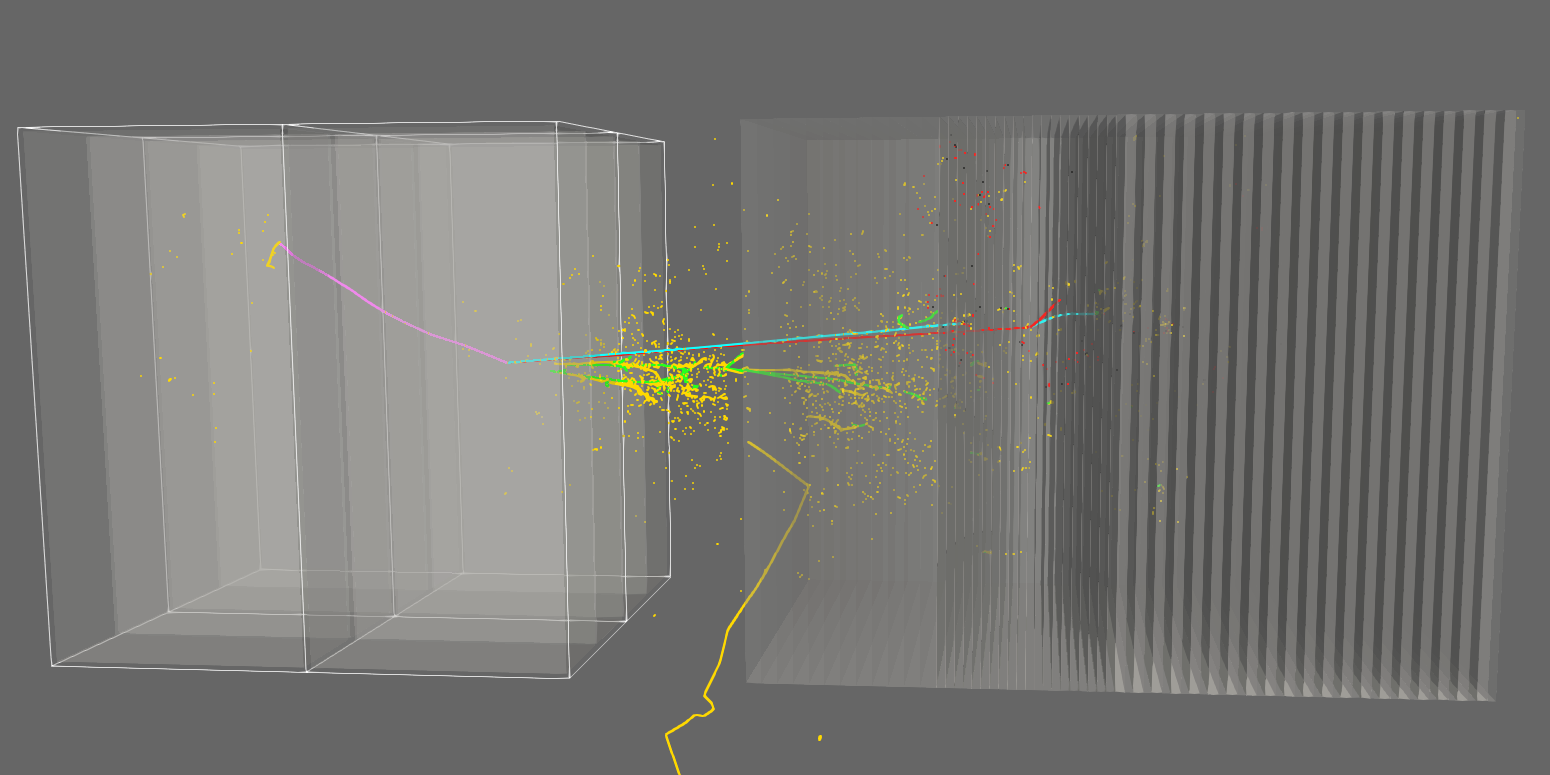
\includegraphics[width=0.8\textwidth]{{plots/Event_Displays_2x2_MINERvA/MINERvA_full_e70_rectangle_crop}.png}
  \caption{Example simulated event for a 7.0 GeV $\nu_{\mu}$--argon charged-current interaction, in which particles not contained in the ArgonCube 2x2 enter the scintillator block detector. Energy deposits are color-coded according to the particle type: $\pi^{\pm}$ --- blue; $\mu^{\pm}$ --- purple; $e^{+}$ --- green; $e^{-}$ --- yellow; proton --- red; recoiling nuclei --- black. The event vertex was randomly placed inside the active volume of the 2x2 Demonstrator module.}
  \label{fig:2x2+MINERvA_event}
\end{figure}

For the studies shown in this section, a simulation was performed approximating the downstream MINERvA central tracking region with a box of scintillator, and the ArgonCube 2x2 Demonstrator module upstream of the shortened MINERvA detector. Neutrino interactions are generated in the ArgonCube active volume, and propagated through an approximation of the ArgonCube 2x2 demonstrator and partial MINERvA detector with a Geant4-based program.  The MINERvA detector is approximated by a rectangular box, \SI[product-units=repeat]{1.4x1.4}{\metre\squared} in the dimensions transverse to the beam.  The simulation includes the most downstream 12 modules (24 planes) of the tracker region, as well as the full downstream ECAL and HCAL regions.  The rectangular box represents the central part of the MINERvA inner detector, and is large enough to cover the entire ArgonCube active volume. An example event is shown in Figure~\ref{fig:2x2+MINERvA_event}, and can be compared with 2x2 only events in Figures~\ref{fig:argonbox_event_display} and~\ref{fig:leaky_event}. Note that this simulation only included the ArgonCube cryostat and MINERvA detector components, no material was included outside these (so escaping particles simply leave without ever re-interacting). This is unlike the previously described ArgonBox simulation, where a large box of argon was simulated (so escaping particles still re-interact). Events were again distributed uniformly throughout the ArgonCube active volume.

In the following, we discuss potential detector physics studies, or improvements to detector physics studies previously discussed in the ArgonCube 2x2-only case (in Section~\ref{sec:detector-physics-studies}), incorporating elements of the MINERvA detector downstream of the ArgonCube 2x2 module.

\subsubsection{Track matching}
All DUNE ND designs considered in Ref.~\cite{dune_ndcsg} include some fast scintillator component, downstream of the LAr ArgonCube component, and downstream of a low-density GAr TPC tracker, to tag escaping particles, photons, and possibly neutrons. There is a significant reconstruction challenge in matching the escaping tracks from the LAr component, with the signals in the scintillator, given the slow charge readout in the LAr TPC, and the high multiplicity DUNE-ND environment.

\begin{figure}[htb]
  \centering
  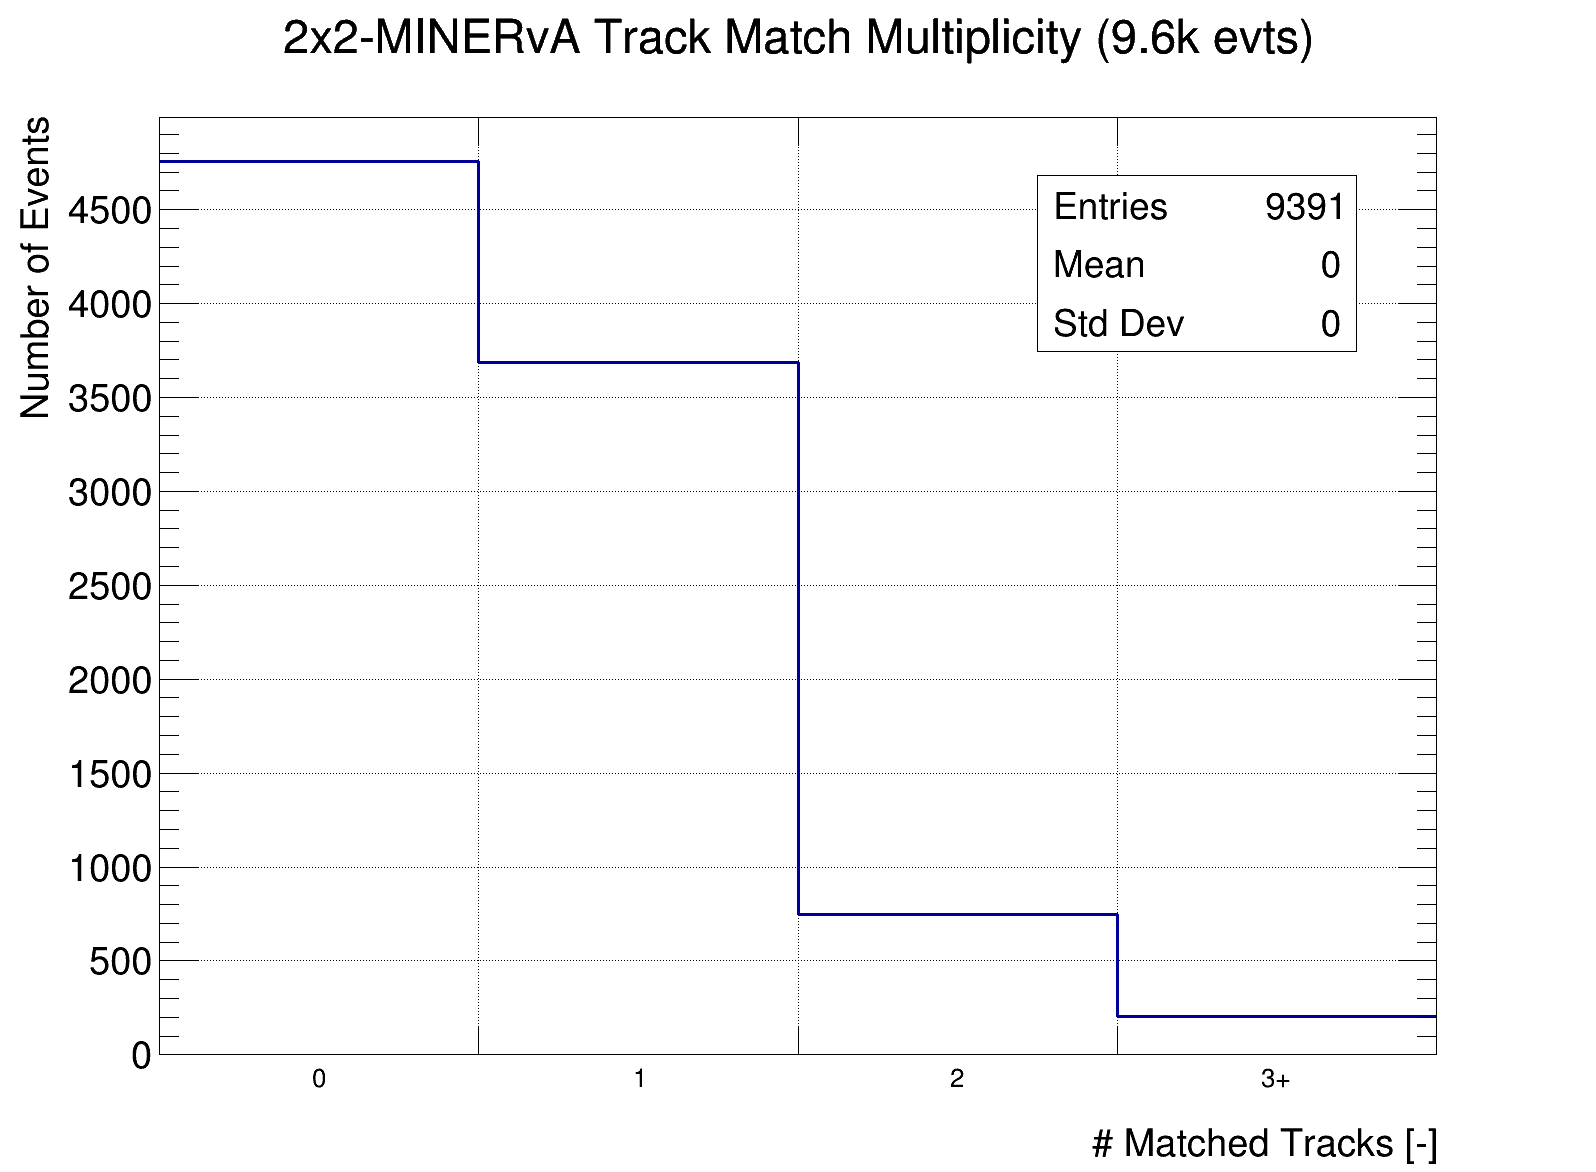
\includegraphics[width=0.6\textwidth]{plots/2x2_minerva_plots/track_mathch_multiplicity.png}
  \caption{Simulated number of true tracks produced by simulated GENIE interactions in the ArgonCube 2x2 active volume, which deposit energy in both the 2x2 module, and the MINERvA component positioned downstream of the 2x2.}
  \label{fig:track_multiplicity_min}
\end{figure}
Many tracks produced in the LAr volume are not contained by the ArgonCube 2x2 module, and the majority will escape downstream. In Figure~\ref{fig:hadronic_containment}, the multiplicity of tracks which deposit charge in both the ArgonCube 2x2 module and the MINERvA component, included in the simulation described above, are shown. Full DUNE-ND events are likely to have an even higher LAr to scintillator track multiplicity due to the pile-up in the much larger 35 t ArgonCube LAr detector. But it is clear from Figure~\ref{fig:track_multiplicity_min} that including MINERvA elements in the ProtoDUNE-ND tests would provide useful data with which to start tackling this reconstruction problem.

\begin{figure}[htb]
  \centering
  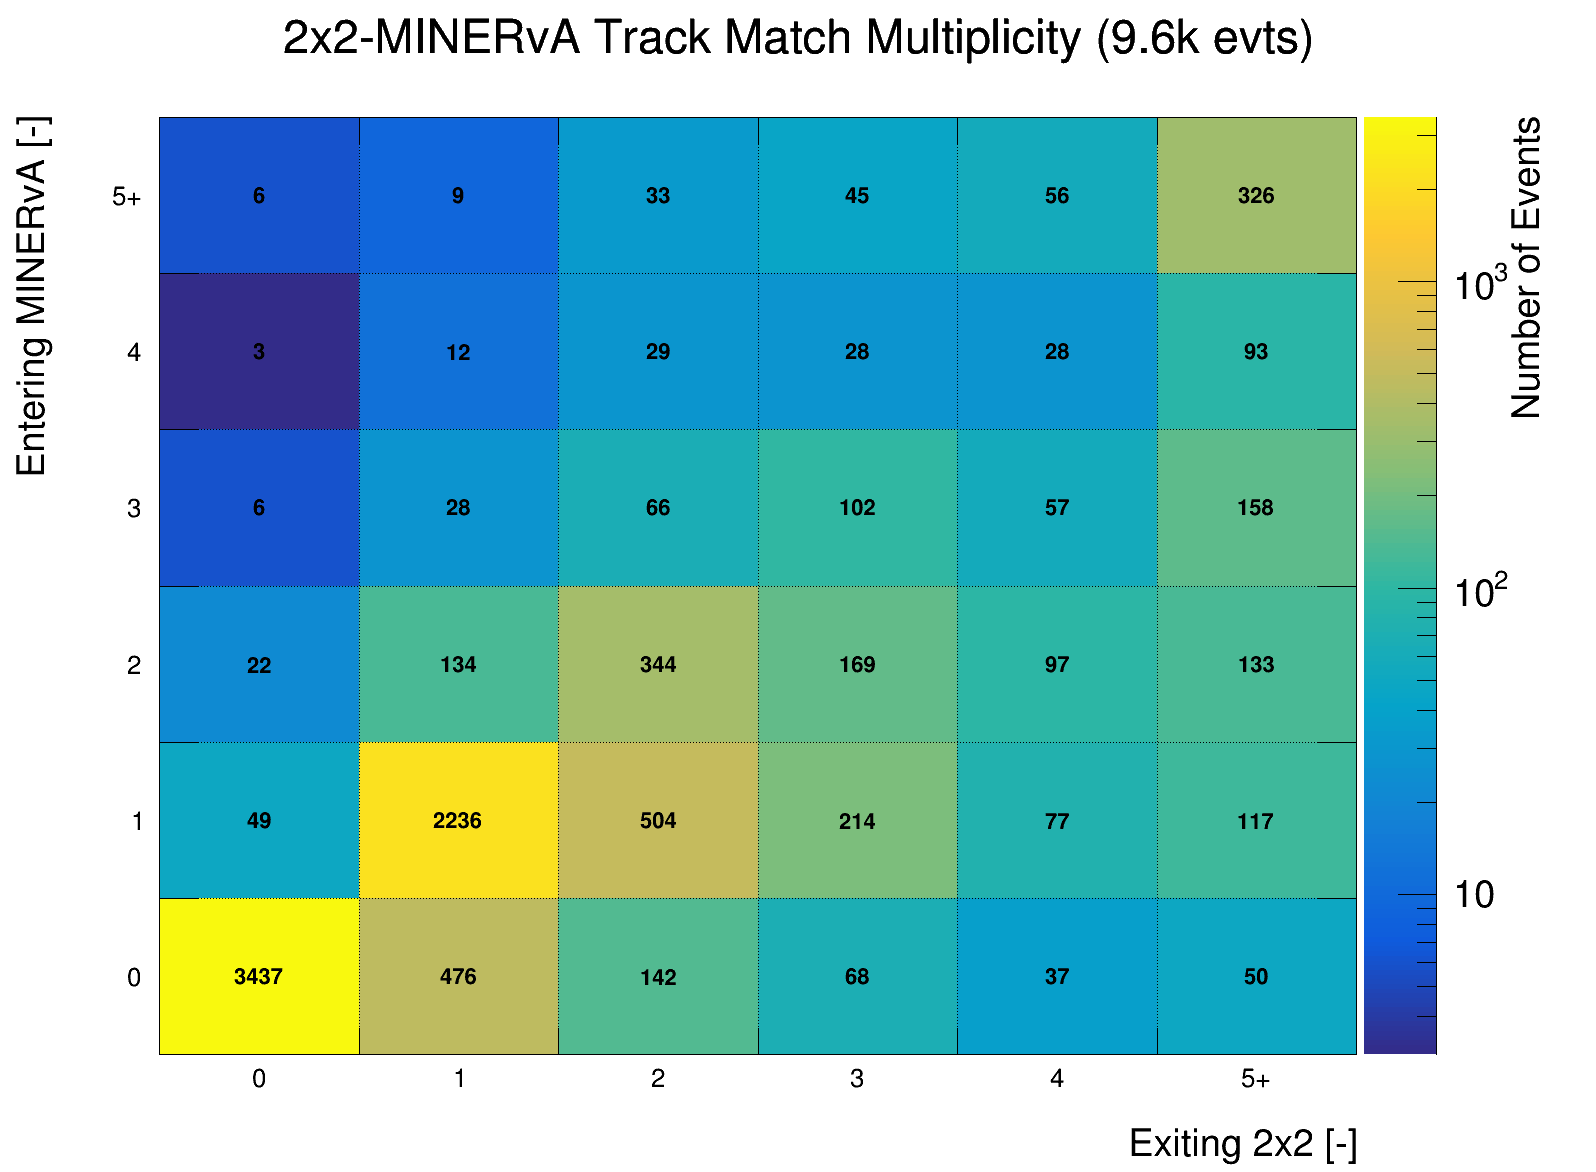
\includegraphics[width=0.6\textwidth]{plots/2x2_minerva_plots/track_mathch_topo.png}
  \caption{Simulated number of true tracks produced by simulated GENIE interactions in the ArgonCube 2x2 active volume, which exit the downstream face of the 2x2 module, relative to the number of tracks which enter the upstream face of the downstream MINERvA component, event by event.}
  \label{fig:track_multiplicity_topo}
\end{figure}
As can be seen from the event display shown in Figure~\ref{fig:2x2+MINERvA_event}, events in which tracks escaping the 2x2 active volume may re-interact in the surrounding LAr bath before entering the MINERvA component included in this simulation, thus making the event more confusing, and difficult to assess reconstruction performance with. Figure~\ref{fig:track_multiplicity_topo} shows the multiplicity of tracks exiting the downstream face of the 2x2 active volume downstream, compared with the number of tracks entering the upstream face of the MINERvA component included in the simulation. The distribution is fairly diagonal, suggesting that although complicated event topologies exist, the events will not be too confused to use for these studies. Note also that this problem could be dramatically reduced by partially instrumenting the dead region between the two detectors.

\subsubsection{Acceptance studies}
\label{sec:minerva-acceptance}
The inclusion of MINERvA in ProtoDUNE-ND will improve the acceptance of particles for various studies. Here, we show how the efficiency for contained events compares for the 2x2+MINERvA setup desribed above, with MINERvA components located downstream of the ArgonCube 2x2 Demonstrator module, and for the 2x2-only case.

\begin{figure}[htb]
  \centering
  \subfloat[2x2-only]    {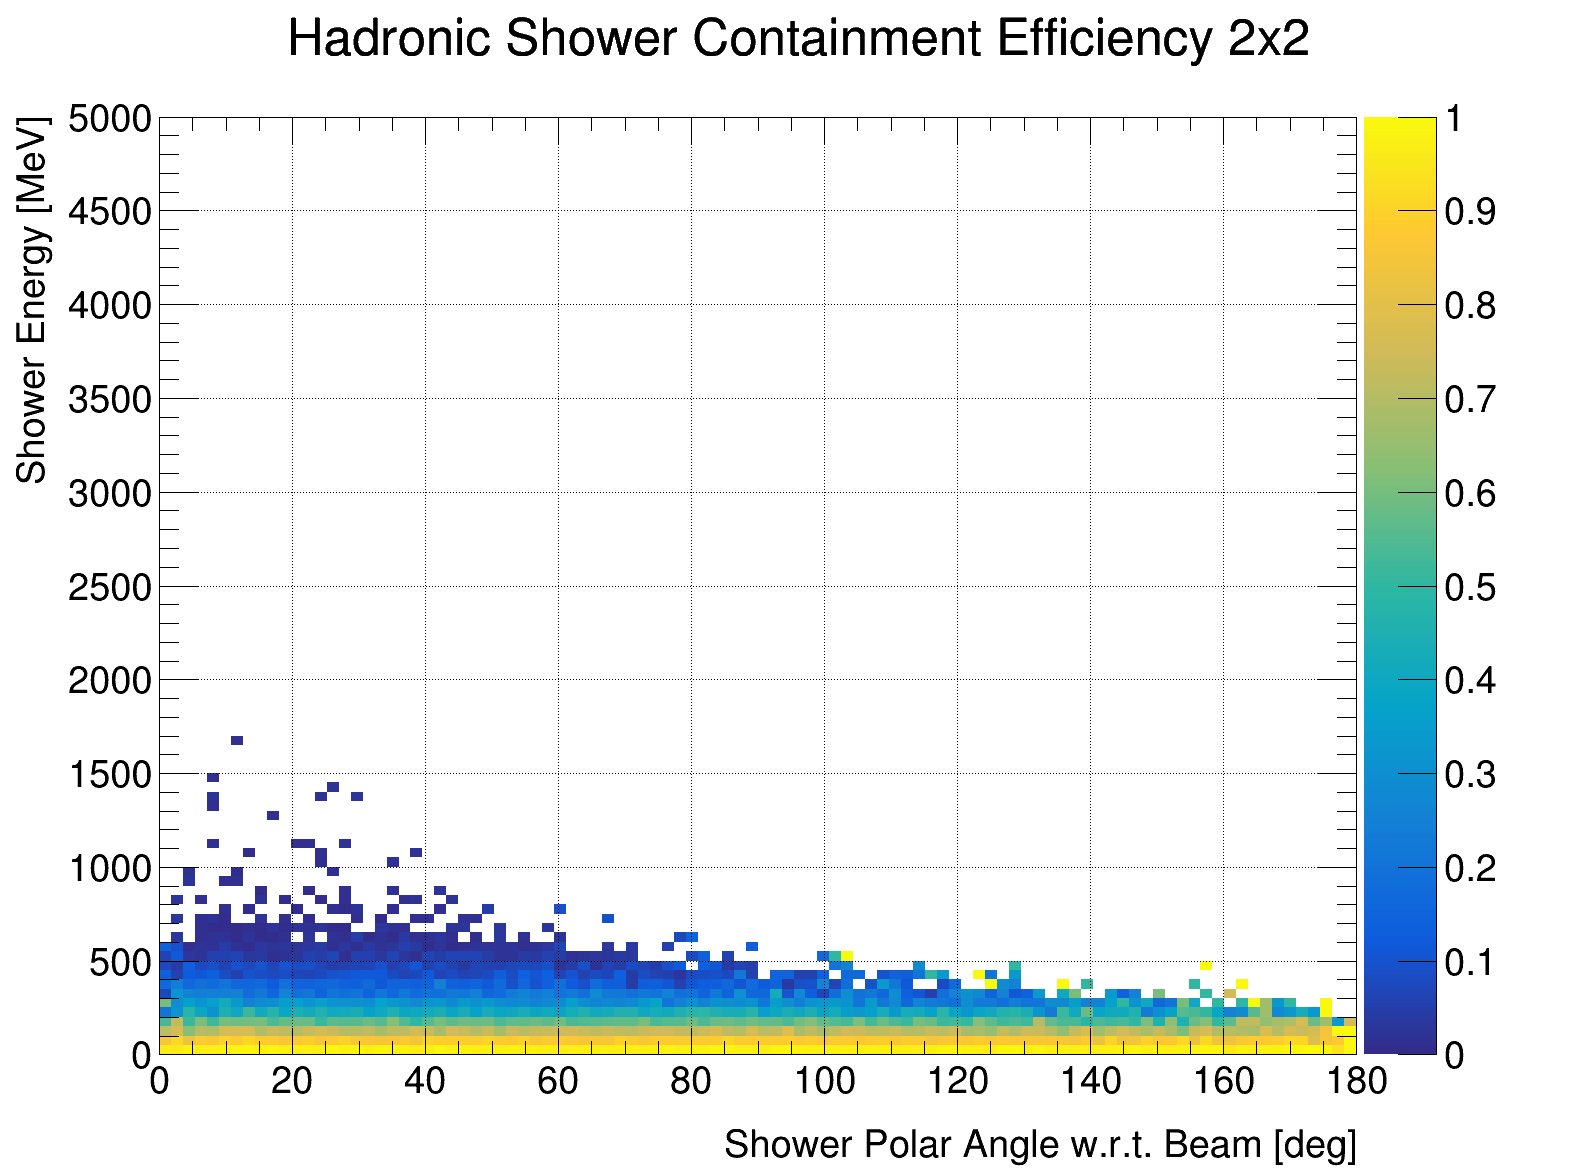
\includegraphics[width=0.45\textwidth]{plots/2x2_minerva_plots/H_cont_eff_2x2.png}}
  \subfloat[2x2+MINERvA] {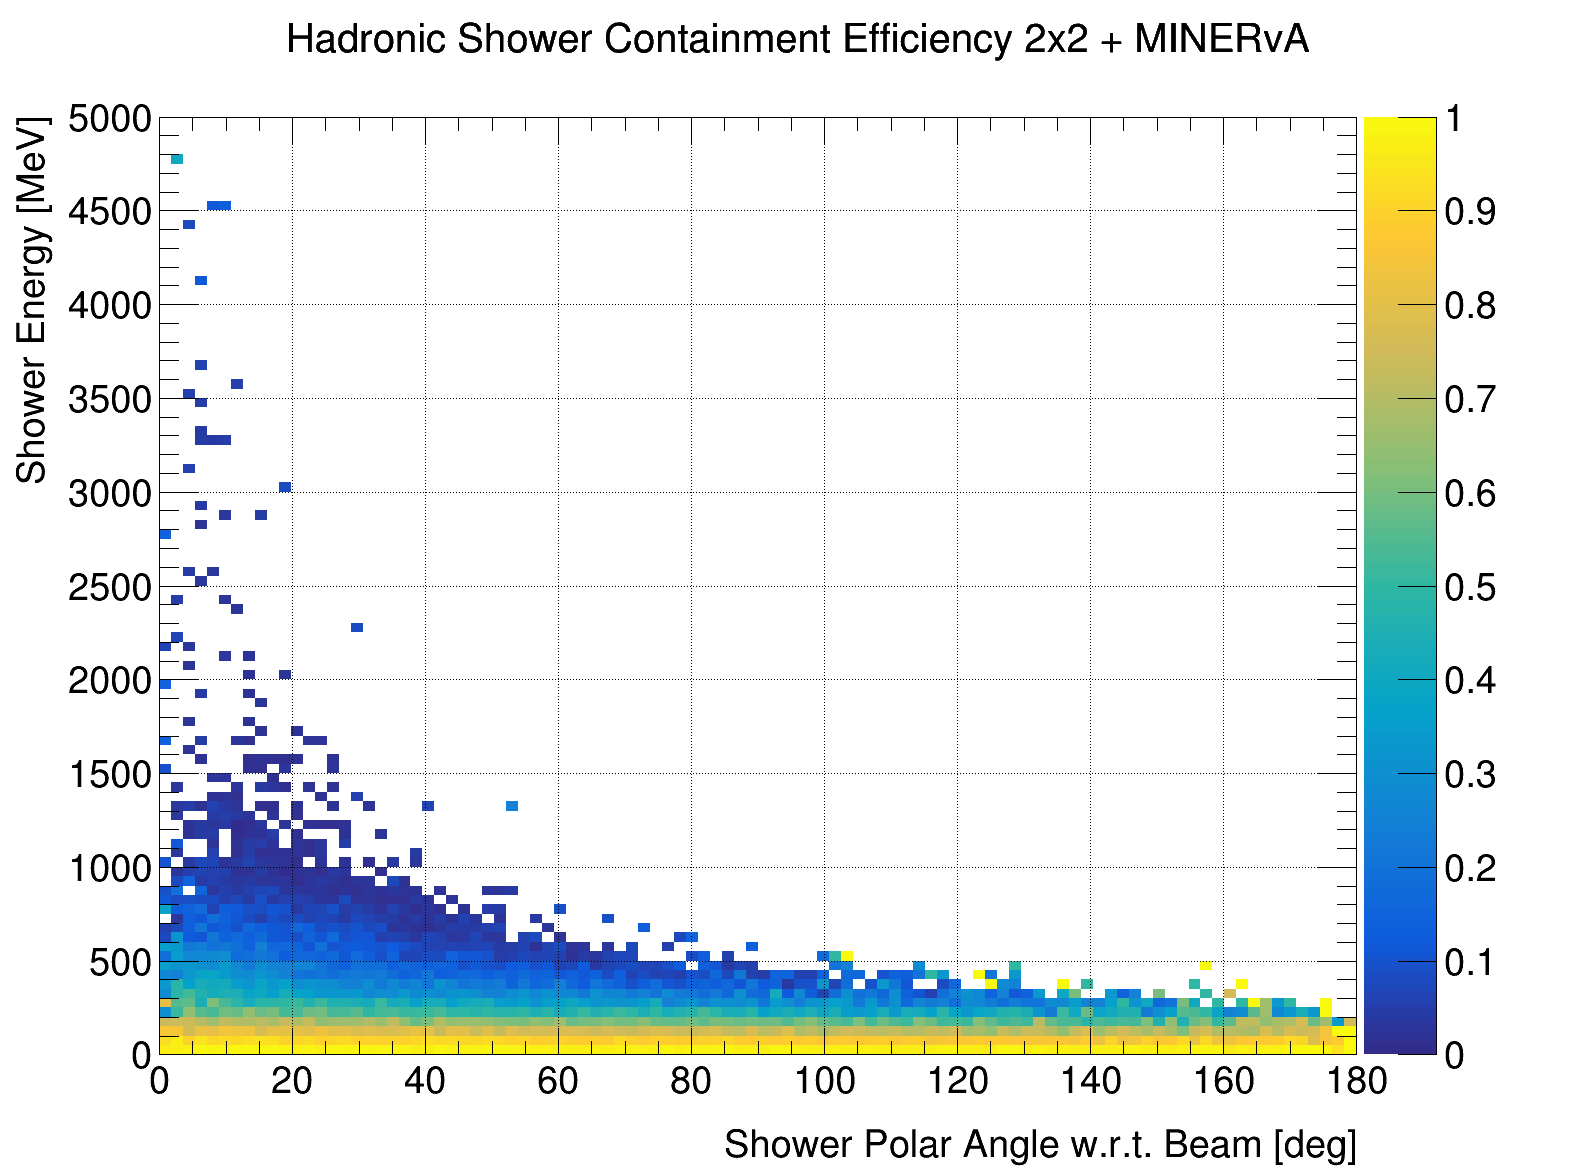
\includegraphics[width=0.45\textwidth]{plots/2x2_minerva_plots/H_cont_eff_2x2_MINERvA.png}}
  \caption{Efficiency for containing hadronic showers, in the 2x2-only, and 2x2+MINERvA, as a function of hadronic shower energy and angle w.r.t the incoming neutrino direction. Containment is defined as $\geq$90\% of the energy being deposited in an active volume of a detector.}
  \label{fig:hadronic_containment}
\end{figure}
In Figure~\ref{fig:hadronic_containment}, the containment of hadron-induced showers is shown as a function of the true energy of the shower, and its angle w.r.t the incoming neutrino beam direction. Showers are defined as being contained when $\geq$90\% of the true energy of the shower is deposited inside the active 2x2 volume, or the MINERvA component if applicable. As expected, including a MINERvA component downstream of the 2x2 module increases the efficiency for angles $\theta \lesssim 30^{\circ}$, which dramatically increases the containment of high energy $E \gtrsim 0.5$ GeV hadronic showers, which tend to be forward-going.

\begin{figure}[htb]
  \centering
  \subfloat[2x2-only]    {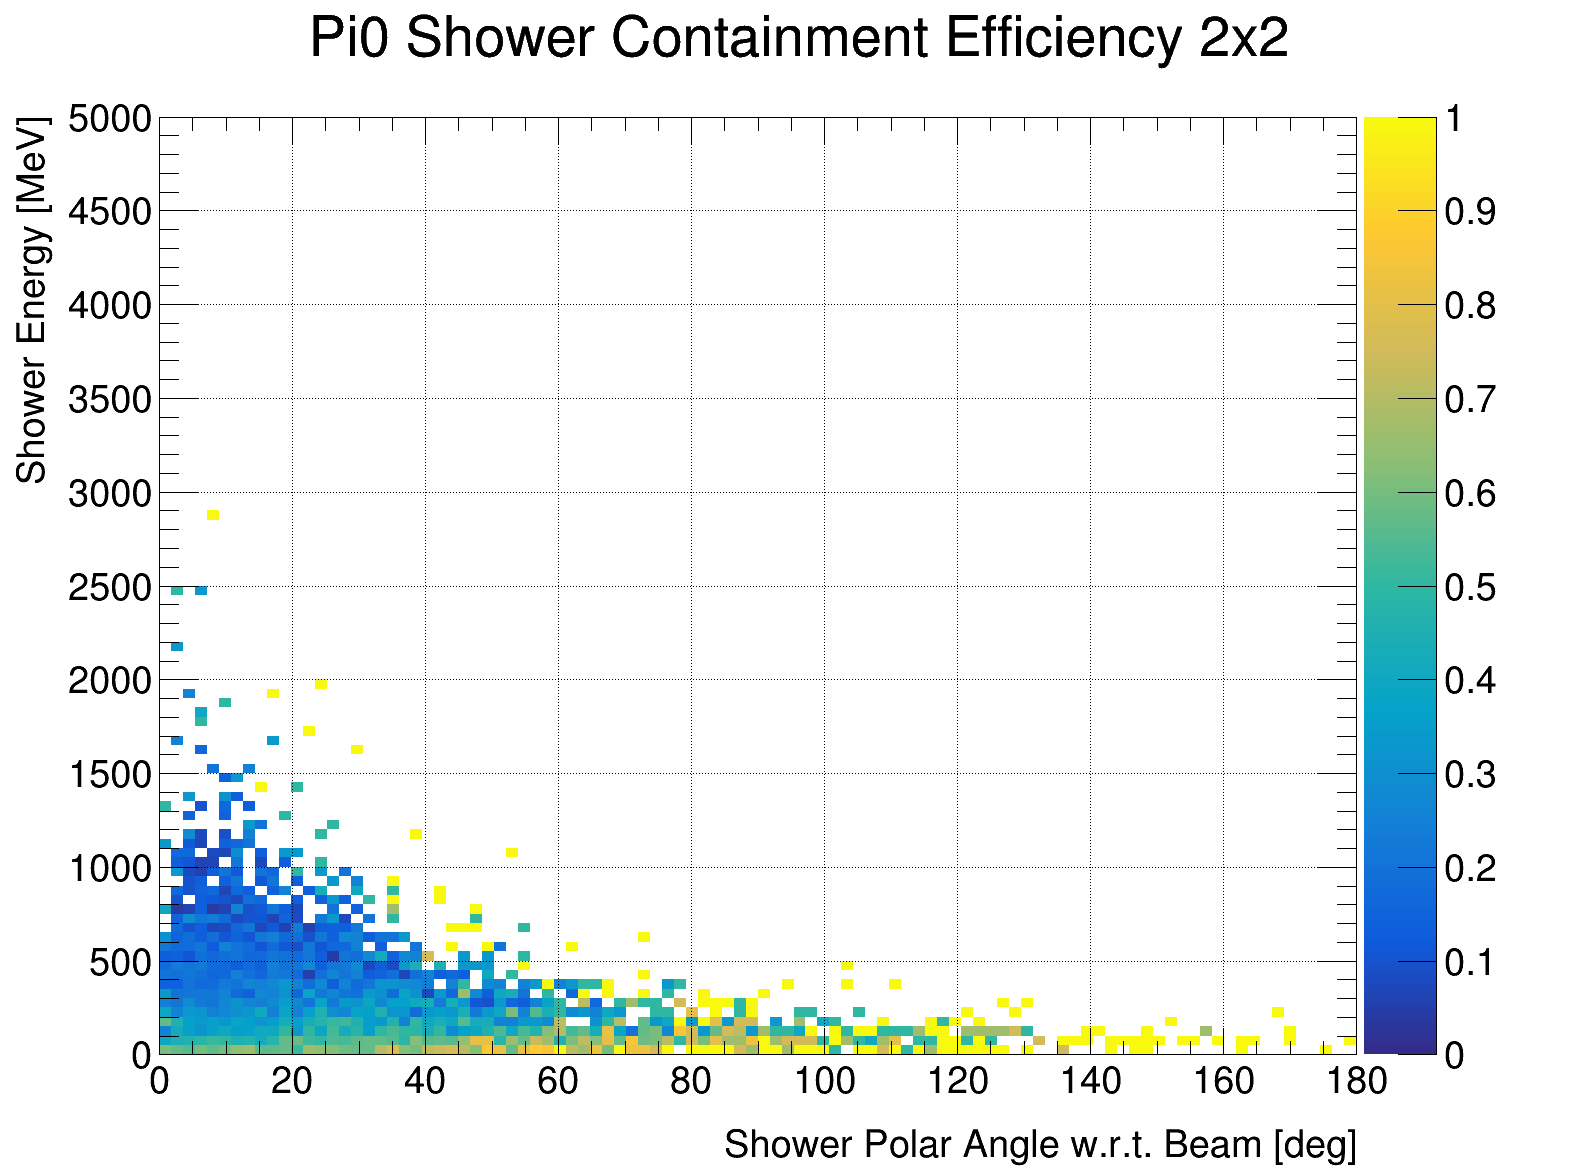
\includegraphics[width=0.45\textwidth]{plots/2x2_minerva_plots/Pi0_cont_eff_2x2.png}}
  \subfloat[2x2+MINERvA] {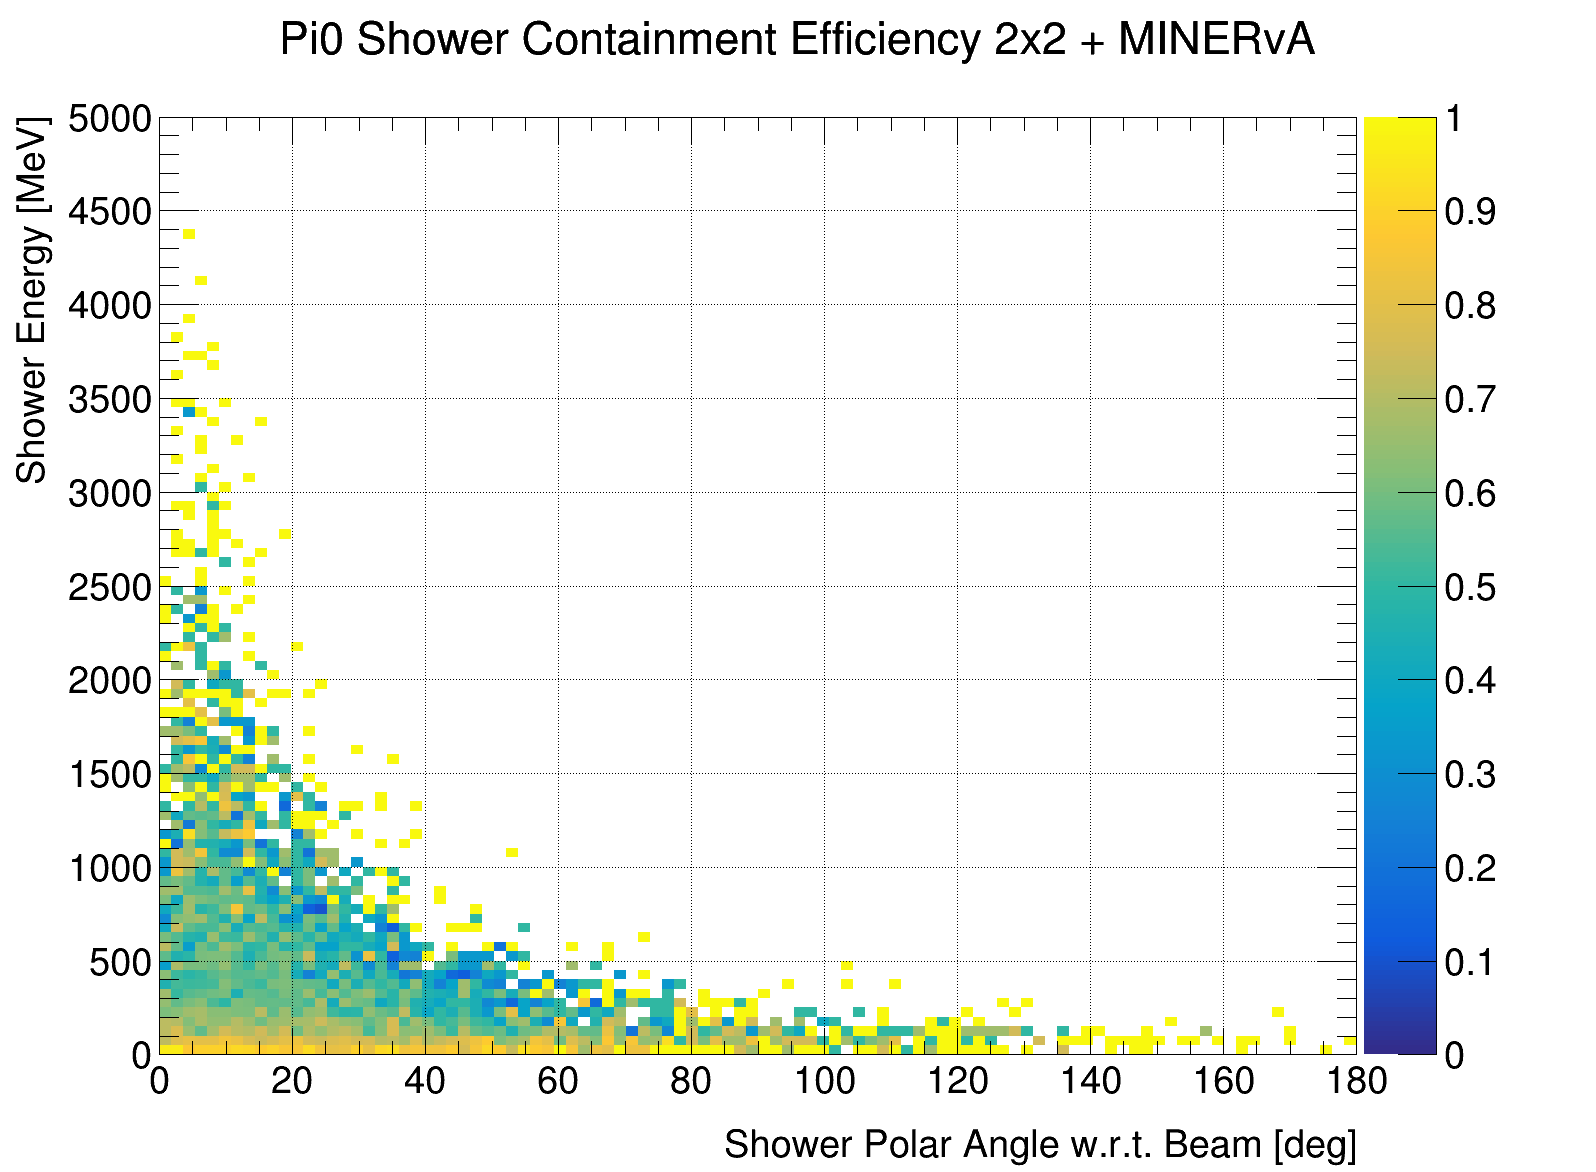
\includegraphics[width=0.45\textwidth]{plots/2x2_minerva_plots/Pi0_cont_eff_2x2_MINERvA.png}}
  \caption{Efficiency for containing both photon-induced showers from $\pi^{0}$ decays, in the 2x2-only, and 2x2+MINERvA, as a function of the $\pi^{0}$ kinetic energy and angle w.r.t the incoming neutrino direction. Containment is defined as $\geq$90\% of the energy being deposited in an active volume of a detector.}
  \label{fig:pi0_containment}
\end{figure}
As discussed previously in this note, as the 2x2 module will not be placed in a test beam prior to installation in the NuMI beam at Fermilab, measurements in which the energy scale of the 2x2 can be calibration will be vital to assess the quality of energy reconstruction in the detector. The containment of both photons from a $\pi^{0}$ decay provides an appropriate in situ measurment of the energy reconstruction capabilities. In Figure~\ref{fig:pi0_containment}, the efficiency to contain 90\% of the energy from both photon-induced showers from a $\pi^{0}$ decay within the active volume of the 2x2, or the MINERvA component if relevant, is shown as a function of the $\pi^{0}$ kinetic energy and angle w.r.t the incoming neutrino beam. There is a significant increase in efficiency for all kinetic energies above a few hundred MeV, particularly for high energy ($E_{\pi^{0}} \gtrsim 1$ GeV) pions, which are produced in the forward direction. Although the dead space between the ArconCube 2x2 active volume and the MINERvA component complicates this picture somewhat, it is clear that including a large portion of MINERvA would give much greater statistics for this benchmark test of the ArgonCube detector performance.

\subsubsection{Neutron tagging studies}

\begin{figure}[htb]
  \centering
  \subfloat[2x2]    {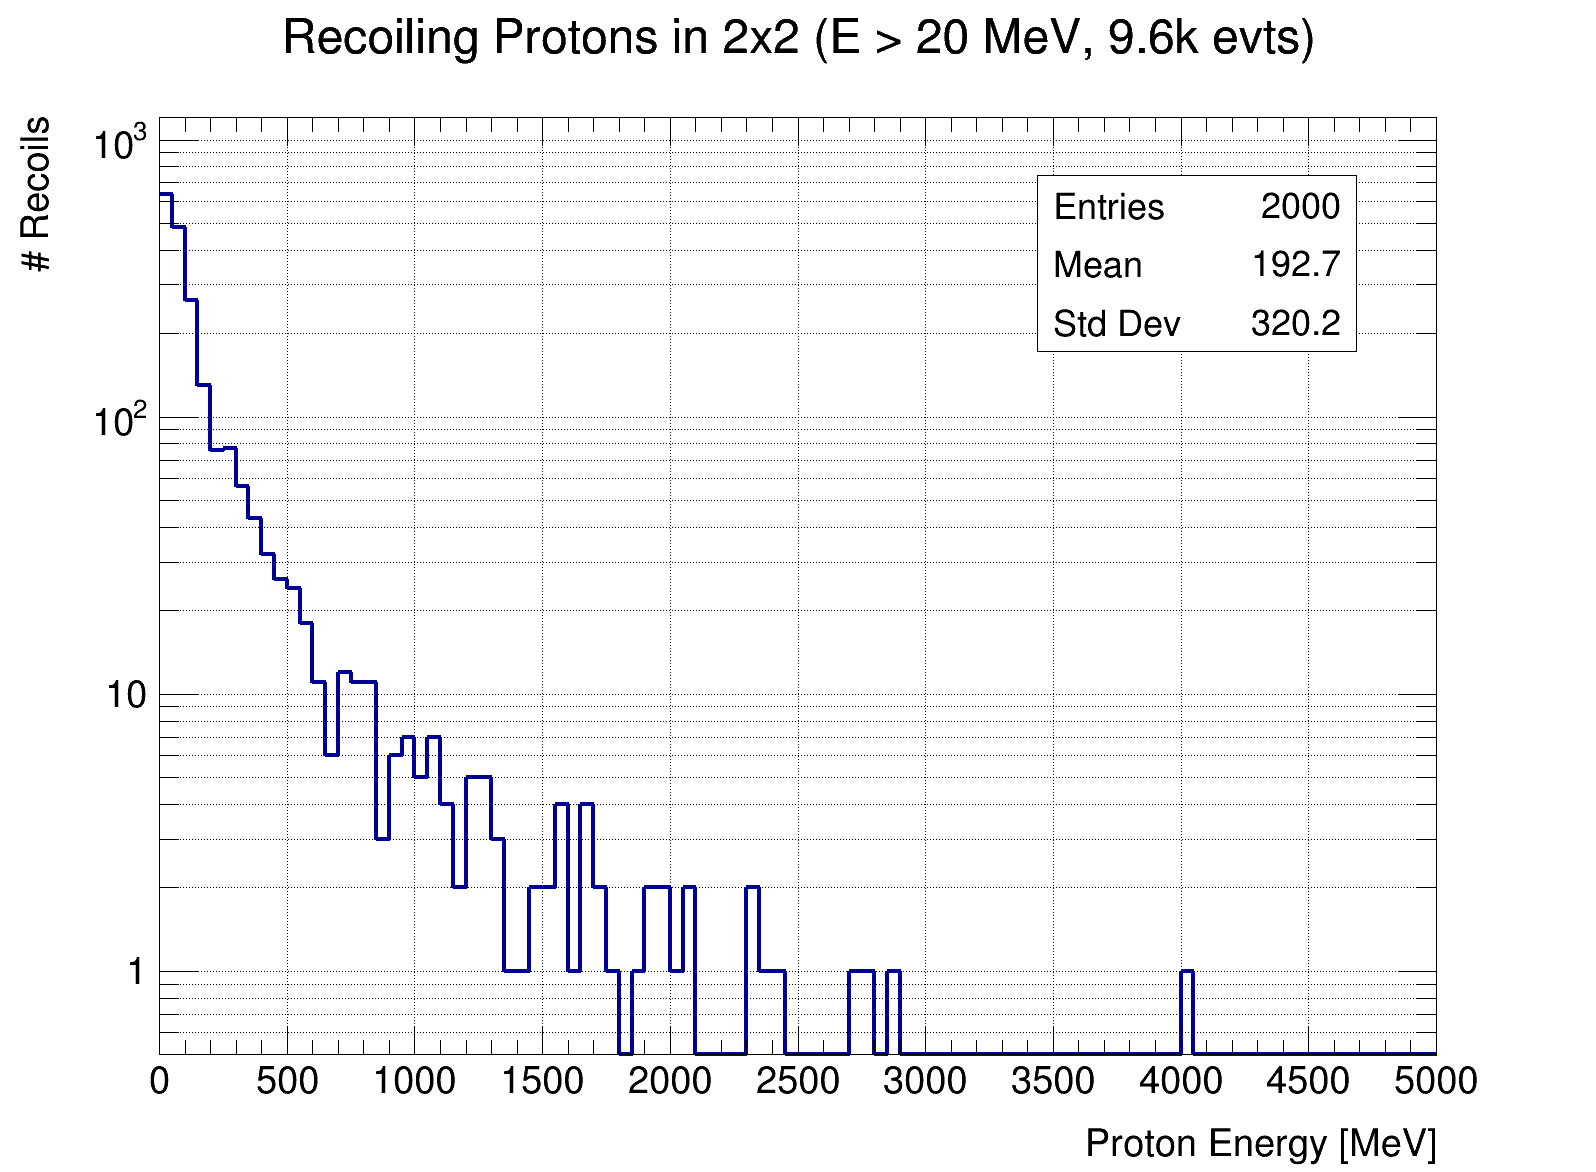
\includegraphics[width=0.45\textwidth]{plots/2x2_minerva_plots/recoils_vs_E_proton_2x2.png}}
  \subfloat[MINERvA] {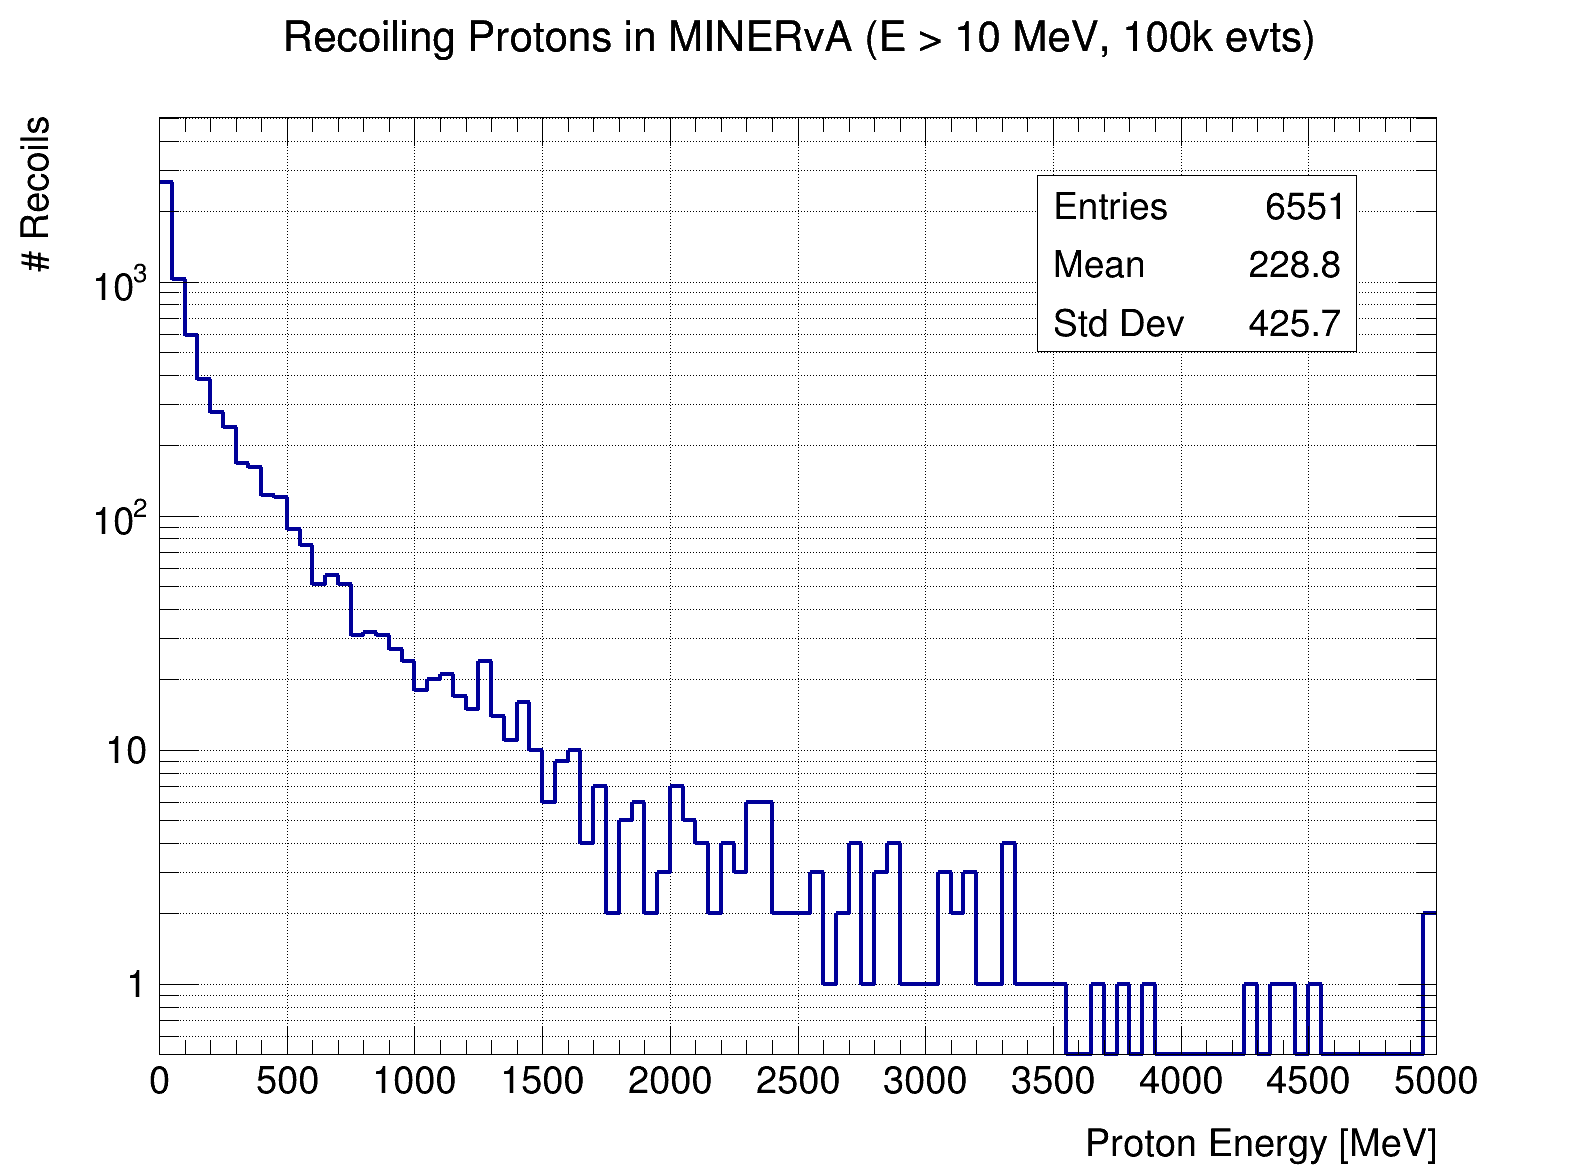
\includegraphics[width=0.45\textwidth]{plots/2x2_minerva_plots/recoils_vs_E_proton_MINERvA.png}}
  \caption{Number of neutron-induced proton recoils as a function of proton energy, which originate from an interaction vertex in the 2x2 active volume, seen in both the 2x2 ative volume, and the downstream MINERvA detector.}
  \label{fig:neutron_tag_minerva}
\end{figure}

As discussed in Section~\ref{sec:2x2_neutron}, one key detector physics goal with ProtoDUNE-ND is to determine whether neutron-induced proton recoils can be identified in a LAr TPC, specifically in ArgonCube. The ability to identify and measure neutrons produced in neutrino interactions is of great interest to DUNE.  At the far detector recoil protons can be identified and easily associated to the neutrino interaction.  However, at the near detector, confusion due to multiple neutrino interactions in the same beam spill poses a unique challenge.  Because neutrons can travel $\mathcal{O}\left(1\right)\,\mathrm{m}$ in LAr without interacting, and proton recoils from fast neutrons typically deposit energy on a single pixel and thus contain no directionality, event association is not possible without matching the charge deposit to an ArCLight optical flash with fast timing resolution.
 
Additionally, it may be possible to measure the neutron energy from time of flight in the DUNE ND using the ECAL with very fast, sub-nanosecond timing resolution. This will require matching muon tracks from either the LAr or HPGAR TPCs to hits in the ECAL to reconstruct the neutrino interaction vertex time with high precision, and also identify and timestamp a subsequent neutron interaction in the scintillator tiles of the ECAL. This would give the DUNE ND unprecedented ability to make measurements of the neutron energy spectrum in neutrino-argon interactions. This technique has not been tested in a high rate environment. Because the neutrons may propagate for $\mathcal{O}\left(10\right)\,\mathrm{ns}$, even a very fast detector may suffer from confusion due to pile-up.

MINERvA can detect neutron-induced proton recoils down to energies of a few MeV, and measure the 3D position of a recoil with a threshold of 20~MeV.  MINERvA has an established neutron reconstruction and a relatively well-understood detector response.  As shown in Fig. 24, it will be possible to reconstruct neutrons originating in the LAr of the ArgonCube 2x2 Demonstrator by their interactions in MINERvA. The ability to match both muons and neutrons originating in LAr to a fast-timing scintillator detector would be a direct test of the feasibility of this technique in DUNE ND. This has profound impact on the design of the ECAL, which would need to be optimized for both EM and neutron reconstruction if this technique is demonstrated to be viable. 
 
 
\FloatBarrier
\subsection{Repurposing the MINOS Near Detector}
The MINOS ND~\cite{MINOS_NIM} is a magnetic spectrometer formed of \SI{1}{\kilo\tonne} of steel and plastic scintillator. It is located \SI{2.1}{\metre} downstream of MINERvA in the NuMI beam line, and is now controlled by the MINERvA collaboration, and maintained with Fermilab. A schematic of MINOS ND is shown in Figure~\ref{fig:minos_near_detector}, it consists of 282 planes of \SI{2.54}{\centi\metre} thick steel. Only 152 planes are instrumented with scintillator. Each scintillator plane is made of \SI{1}{\centi\metre} thick  and \SI{4.1}{\centi\metre} wide strips. The most upstream 120 planes form the calorimeter region, where every steel plane is instrumented with scintillator in a central region, and every 5th plane is fully instrumented.  In the downstream spectrometer region, there are no partially-instrumented planes and only every 5th plane is instrumented. The calorimeter alone stops a 5~GeV muon, and the calorimeter combined with the spectrometer stops a 10~GeV muon.

\begin{figure}[htb]
	\centering
	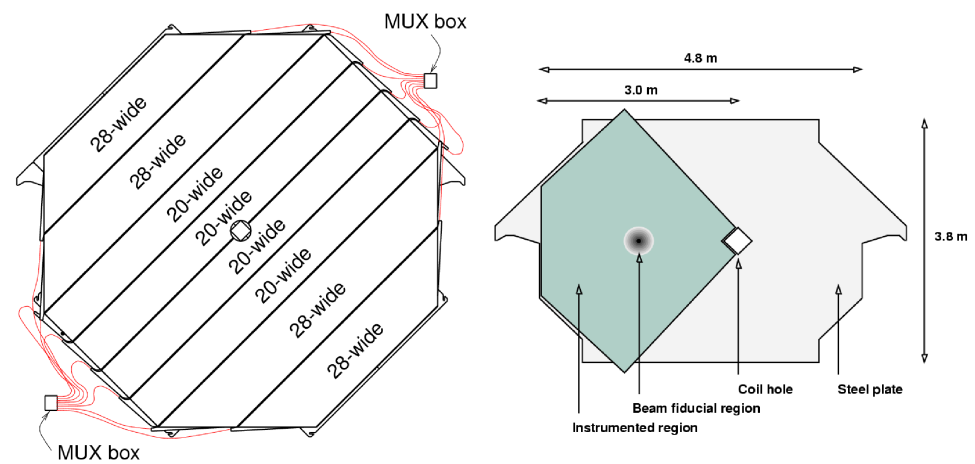
\includegraphics[width=0.9\textwidth]{plots/minos.png}
	\caption{Left: Top view of the MINOS near detector, showing the calorimeter and muon spectrometer (not to scale). Right: transverse view of a near detector plane. The shaded area shows a partially instrumented active scintillator plane and the dashed line within shows the boundary of the fiducial region. The dotted line shows the outline of a fully instrumented scintillator plane. Reproduced from Figure~2 of~\cite{MINOSDetectors}.}
	\label{fig:minos_near_detector}
\end{figure}

As the majority of muons are not contained within the MINERvA volume, and mostly exit downstream, MINERvA currently employ MINOS as a muon spectrometer. Similarly, for ProtoDUNE-ND, the majority of particles will not be contained in the ArgonCube 2x2 volume. Even if MINERvA components are placed downstream of the 2x2 module, the majority of muons will not be contained, making ancilliary physics measurements with ProtoDUNE-ND extremely challenging. Employing MINOS ND as a range finder for ProtoDUNE-ND would allow the muon momentum to be measured, and would allow ProtoDUNE-ND to make much more DUNE-ND-like measurements. If MINOS-ND were to be included downstream, of the MINERvA component, it would also make sense to deploy portions of the MINERvA detector around the ArgonCube cryostat, since the entire MINERvA detector would no longer be needed downstream to maximize momentum sensitivity, making it much easier to tag escaping particles, and to identify through-going cosmics (as alluded to in Section~\ref{sec:cosmic-suppression}), which would make is much easier to calibrate the energy scale in the detector. MINERvA EM scintillator modules could be used to provide vetos for cosmic and rock induced particles entering or exiting the 2x2 cryostat, or to contain side-escaping showers. Ultimately, this would enable a test of the assumption that the DUNE ND does not require a side muon tracker.

Here we discuss such possibilities in brief, and will wait to discover the viability of this project before embarking on more detailed studies. Use of the MINOS ND, in combination with an augmented MINERvA, would allow the reconstruction of the entire properties of an event which occurred in the ArgonCube 2x2 volume. This serves as a proxy for neutrino energy reconstruction, as it would in the full DUNE-ND, and would provide the most thorough calibration of the response of 2x2 possible --- vital, as there are no plans to calibrate the response in a test beam before installation in the MINOS-ND hall at Fermilab.

\subsubsection{Validation of multiple coulomb scattering}

The DUNE ND will employ a downstream tracking detector to measure forward, high-energy muons, and will be sufficiently wide as to contain muons at high angles.  However, for wide-angle muons, tracks will only be contained when the vertex is far from the edges, and will often exit the TPC and not be reconstructed.  This sample could be recovered if the muon momentum can be measured reliably from multiple coulomb scattering (MCS). The far detector will also use MCS for muons which exit the detector.

Such measurements have been carried out in a LAr TPC by MicroBooNE~\cite{Abratenko:2017nki}, although the momentum range is somewhat limited as the only validation sample available is composed of muons which stop in the detector, for which a momentum by range measurement can be made. However, such measurements may be more challenging in a modular TPC such as ArgonCube, where tracks are necessarily broken into segments which are read out separately, and then combined in downstream software.

Although there are only four modules in the ArgonCube 2x2 Demonstrator, each is split into two TPCs, so tracks which exit the downstream face of the 2x2 module may be sampled by up to four independent charge readout planes. With a downstream detector capable of making a precise muon momentum measurement, it would be possible to demonstrate that multiple coulomb scattering will be a viable technique for making momentum measurements in the full ArgonCube deployment in the DUNE ND. Given the hard muon momentum spectrum expected in the NuMI on-axis beam (shown in Figure~\ref{fig:momenta}), it would be hard to make a reliable momentum measurement with a small demonstrator tracker module, or indeed with the MINERvA components proposed in Section~\ref{sec:minerva}, as few would be contained. Such measurements could be made, in the MINOS-ND, which is capable of making momentum measurements for all relevant muon momenta by curvature, or by range.

\subsubsection{Use of MINERvA as a cosmic trigger}
In the discussion in Section~\ref{sec:minerva}, the detector setup maximizes the amount of the MINERvA detector repurposed downstream of the ArgonCube 2x2 module, in order to increase containment in the very forward region, where most particles go. However, if MINOS-ND is also included as part of the ProtoDUNE-ND setup, this imperative is no longer there, and less of MINERvA would be needed downstream. In this case, MINERvA modules could be redeployed to the sides of, and even above, the 2x2 cryostat to act as a cosmic ray or dirt muon tagger, and to tag escaping particles. In practice, these panels could be used to better identify a sample of fully contained neutrino events for the studies outlined in Sections~\ref{sec:minerva-acceptance}. Additionally, these cosmic ray tagging modules could then be used to validate space charge build-up and electric field uniformity studies outlined in Section~\ref{sec:efield}, and the cosmic suppression studies described in Section~\ref{sec:cosmic-suppression}, for which an additional scintillator panel would be required.

\subsection{MINERvA/MINOS running costs}
The estimated labor costs for MINERvA infrastructure support are:
\begin{itemize}
\item 1 person as coordinator and interface with lab computing experts --- 0.5 FTE
\item 1 person as software release and support (Gaudi) --- 0.5 FTE
\item 1 person to monitor keepup --- 0.1-0.25 FTE
\item 2 people for production --- 0.5 FTE (very conservative)
\end{itemize}
Giving a total requirement of 2.1--2.25 FTE, which would have to come from current MINERvA collaborators, not necessarily FNAL employees, who are interested in joining the ProtoDUNE-ND effort. It should be noted that in FY17 MINERvA and MINOS combined used 0.3 FTE from the FNAL Neutrino Division Detector Operations group.

\begin{table}[htbp]
  \centering  
      {\renewcommand{\arraystretch}{1.2}
        \begin{tabular}{cccc}
          \hline\hline
          & & CPU hours & Disk usage (bytes) \\
          \hline
          \multirow{2}{*}{Data} & MINERvA (50\%) & $4.85\times 10^{4}$ & $2.07\times 10^{13}$ \\
          & MINOS & $7.65\times 10^{4}$ & $4\times 10^{12}$ \\
          \hline
          \multirow{2}{*}{MC} & MINERvA (50\%) & $1.8\times 10^{5}$ & $6.3\times 10^{13}$ \\
          & MINOS & $4.5\times 10^{4}$ & $1.3\times 10^{12}$ \\          
          \hline
          \multicolumn{2}{c}{Total} & $3.5\times 10^{5}$ & $8.9\times 10^{13}$ \\
          \hline\hline
      \end{tabular}}  
      \caption{Estimated computing resources required to run MINERvA and the MINOS-ND, assuming that 50\% of MINERvA is retained for ProtoDUNE-ND.}
      \label{tab:minerva-computing}
\end{table}
The expected yearly computing requirement for MINERvA with and without MINOS-ND are shown in Table~\ref{tab:minerva-computing}, assuming that ~50\% of the MINERvA detector is retained and repurposed for ProtoDUNE-ND. Note that it has been assumed that the Monte Carlo production should be ~2$\times$ the data, in keeping with current practice for MINERvA analyses in the NuMI medium energy beam. Note also that the costs in Table~\ref{tab:minerva-computing} do not include those for the ArgonCube 2x2 module. Assuming a cost of \$0.01/CPU hour and \$30/TB, the total cost per year is estimated to be $\sim$\$6000 ($\sim$\$3500 CPU + $\sim$\$2500 disk). Note that in this estimate of computing costs, we have not included the cost of databases and their allocations, or the cost of supporting and maintaining the readout machines.

There are sufficient spare Minder Boards for MINERvA for at least 2 years of operations with the full detector, so there should be plenty of spares given that we would not be using all of the existing MINERvA detector. MINOS front end boards (FEBs) are difficult to replace and prone to failure, however, if the use of MINOS-ND for ProtoDUNE-ND were to be seriously considered, it may be possible to replace the current MINOS FEBs with MINERvA Minder Boards, and still have plenty to spares. This possibility should be seriously considered if the instability of MINOS FEBs are a major issue for this proposal. Of course, the labor cost of such an endeavour would need to be bourne by current MINERvA collaborators wishing to join the DUNE R\&D efforts. 

Finally, the cost of running the detectors themselves has not been considered here. We note that the majority of the power consumption by MINERvA+MINOS-ND is used to run the MINOS-ND magnet. Although the magnet is desirable, it would be possible to use MINOS-ND with the magnet off, at least for some portion of the time, and get momentum estimates by range only.
